\documentclass[11pt,aspectratio=43,usenames,dvipsnames]{beamer}
\usepackage[utf8]{inputenc}
\usepackage{amsmath, amsfonts, amssymb, amsthm}
\usepackage[T1]{fontenc}
% mint: code chuck and syntax highlighting
%% outputdir should change according to pdf build directory
\usepackage[outputdir=build,cache=false]{minted}
\usepackage{lmodern}
\usepackage{xcolor}
\usepackage{setspace}
\usepackage{booktabs}
\usepackage{multirow}
\usepackage{graphicx}
\usepackage{fontawesome}
\usepackage{pgfplots}
\pgfplotsset{compat=newest, scale only axis, width = 10cm}
\pgfplotsset{sciclean/.style={axis lines=left,
        axis x line shift=1em,
        axis y line shift=1em,
        axis line style={-,very thin},
        axis background/.style={draw,ultra thin,gray},
        tick align=outside,
        xtick distance=0.5,
        ytick distance=0.5,
        major tick length=2pt}}
\usepackage{tikz}
\usetikzlibrary{datavisualization, datavisualization.formats.functions}
% \usetikzlibrary{decorations}
\usetikzlibrary{decorations.pathreplacing, intersections}
\usepackage{ulem}
\usepackage{hyperref}
\usepackage{booktabs}
\usepackage{babel}
\usepackage{makecell}
\usepackage[para,online,flushleft]{threeparttable}
\usepackage{pdfpages}
\usepackage{tcolorbox}
\usepackage{bm}
\usepackage{appendixnumberbeamer}
\usepackage{natbib}
\usepackage{caption}
\captionsetup[figure]{labelformat=empty}% redefines the caption setup of the figures environment in the beamer class.
\usetheme[compress]{Boadilla}
\usecolortheme{default}
\useoutertheme{miniframes}
\usefonttheme[onlymath]{serif}

\newcommand{\jump}[2]{\hyperlink{#1}{\beamerbutton{#2}}}
\newcommand{\orange}[1]{\textcolor{orange}{#1}}
\newcommand{\red}[1]{\textcolor{red}{#1}}
\newcommand{\blue}[1]{\textcolor{blue}{#1}}
\newcommand{\green}[1]{\textcolor{OliveGreen}{#1}}

\renewcommand{\square}{\scalebox{0.7}{$\blacksquare$ \hspace{0.5em}}}
\setbeamertemplate{itemize item}{\raisebox{0.1em}{\scalebox{0.7}{$\blacksquare$}}}
\setbeamertemplate{itemize subitem}[circle]
\setbeamertemplate{itemize subsubitem}{--}
\setbeamercolor{itemize item}{fg=black}
\setbeamercolor{itemize subitem}{fg=black}
\setbeamercolor{itemize subsubitem}{fg=black}
\setbeamercolor{item projected}{bg=darkgray,fg=white}
\definecolor{blue}{rgb}{0.2, 0.2, 0.7}
\setbeamercolor{alerted text}{fg=blue}
\setbeamertemplate{enumerate items}[circle]


\setbeamertemplate{headline}{}

%==========================================
\let\olditemize=\itemize
\let\endolditemize=\enditemize
\renewenvironment{itemize}{\olditemize \itemsep1em}{\endolditemize}
\let\oldenumerate=\enumerate
\let\endoldenumerate=\endenumerate
\renewenvironment{enumerate}{\oldenumerate \itemsep1em}{ \endoldenumerate}

\DeclareMathOperator*{\argmax}{\arg\!\max}
\DeclareMathOperator*{\E}{\mathbb{E}}
\DeclareMathOperator*{\var}{\rm Var}
\DeclareMathOperator*{\cov}{\rm Cov}

\theoremstyle{definition}
\newtheorem{assume}{Assumption}
\newtheorem{lem}{Lemma}
\newtheorem{proposition}{Proposition}
\newtheorem{thm}{Theorem}
\newtheorem{corol}{Corollary}

\AtBeginSection[]{
  \begin{frame}[noframenumbering]
  \vfill
  \centering
  \begin{beamercolorbox}[sep=8pt,center,shadow=true,rounded=true]{title}
    \usebeamerfont{title}\insertsection\par%
  \end{beamercolorbox}
  \vfill
  \end{frame}
}

\begin{document}
    \title[Unit 3]{Unit 3 \\ Scarcity, Work and Choice}
    \author[Hui-Jun Chen]{Hui-Jun Chen}
    \institute[OSU]{The Ohio State University}
    % \date{\today}
    \date{\today}
    \setbeamertemplate{navigation symbols}{}
    \setstretch{1.2}

%-------------------------------------------------------
{
%	\usebackgroundtemplate{\includegraphics[width=1\paperwidth]{../EveningSky_cropped_edit43_bright.jpg}}
    \begin{frame}
% \vspace{3em}
        \centering
%		{\footnotesize 	ECON 4002 Intermediate Macroeconomic Theory}
        \maketitle
% \vspace{-1.5em}
% \centering
% \includegraphics[width=0.55\linewidth]{Pictures/houses.jpeg}


    \end{frame}
}

% -------------------------------------------
\setbeamertemplate{headline}
{
\setbeamercolor{section in head/foot}{fg=black, bg=white}
\vskip1em \tiny \insertsectionnavigationhorizontal{1\paperwidth}{\hspace{0.50\paperwidth}}{}
}
%------------------------------------------

\section[Intro]{Introduction}
\label{sec:Introduction}

\begin{frame}{Introduction}
\label{slide:Introduction}
    In this Unit I start to introduce consumer theory, i.e., \alert{individual behavior}.

    Why?! $ \Rightarrow  $ \textbf{Macro needs Micro foundation}, since
    \begin{itemize}
        \item aggregate behavior is the sum of individual decisions
        \item \alert{Lucas' critique}: structures of economies \alert{change} w/ policies b/c \alert{individual decision} changed
        \item Need to know effect on \alert{individual behavior} to know the aggregate effect!
        \item E.g. Two forces / reactions of COVID stimulus policy:
        \begin{enumerate}
            \item $ \Rightarrow  $ workers have \alert{less} incentive to work $ \Rightarrow  $ unemployment $ \uparrow  $ $ \Rightarrow  $ exacerbate recession
            \item $ \Rightarrow  $ funding $ \uparrow  $ $ \Rightarrow  $ firms have \alert{more} incentive to hire workers $ \Rightarrow  $ mitigate recession
        \end{enumerate}
    \end{itemize}
\end{frame}

\begin{frame}{This Unit}
\label{slide:This_Unit}
    \begin{center}
        Hours of work is different across countries and over time. Why?
    \end{center}
    \begin{columns}
        \begin{column}{0.5\textwidth}
            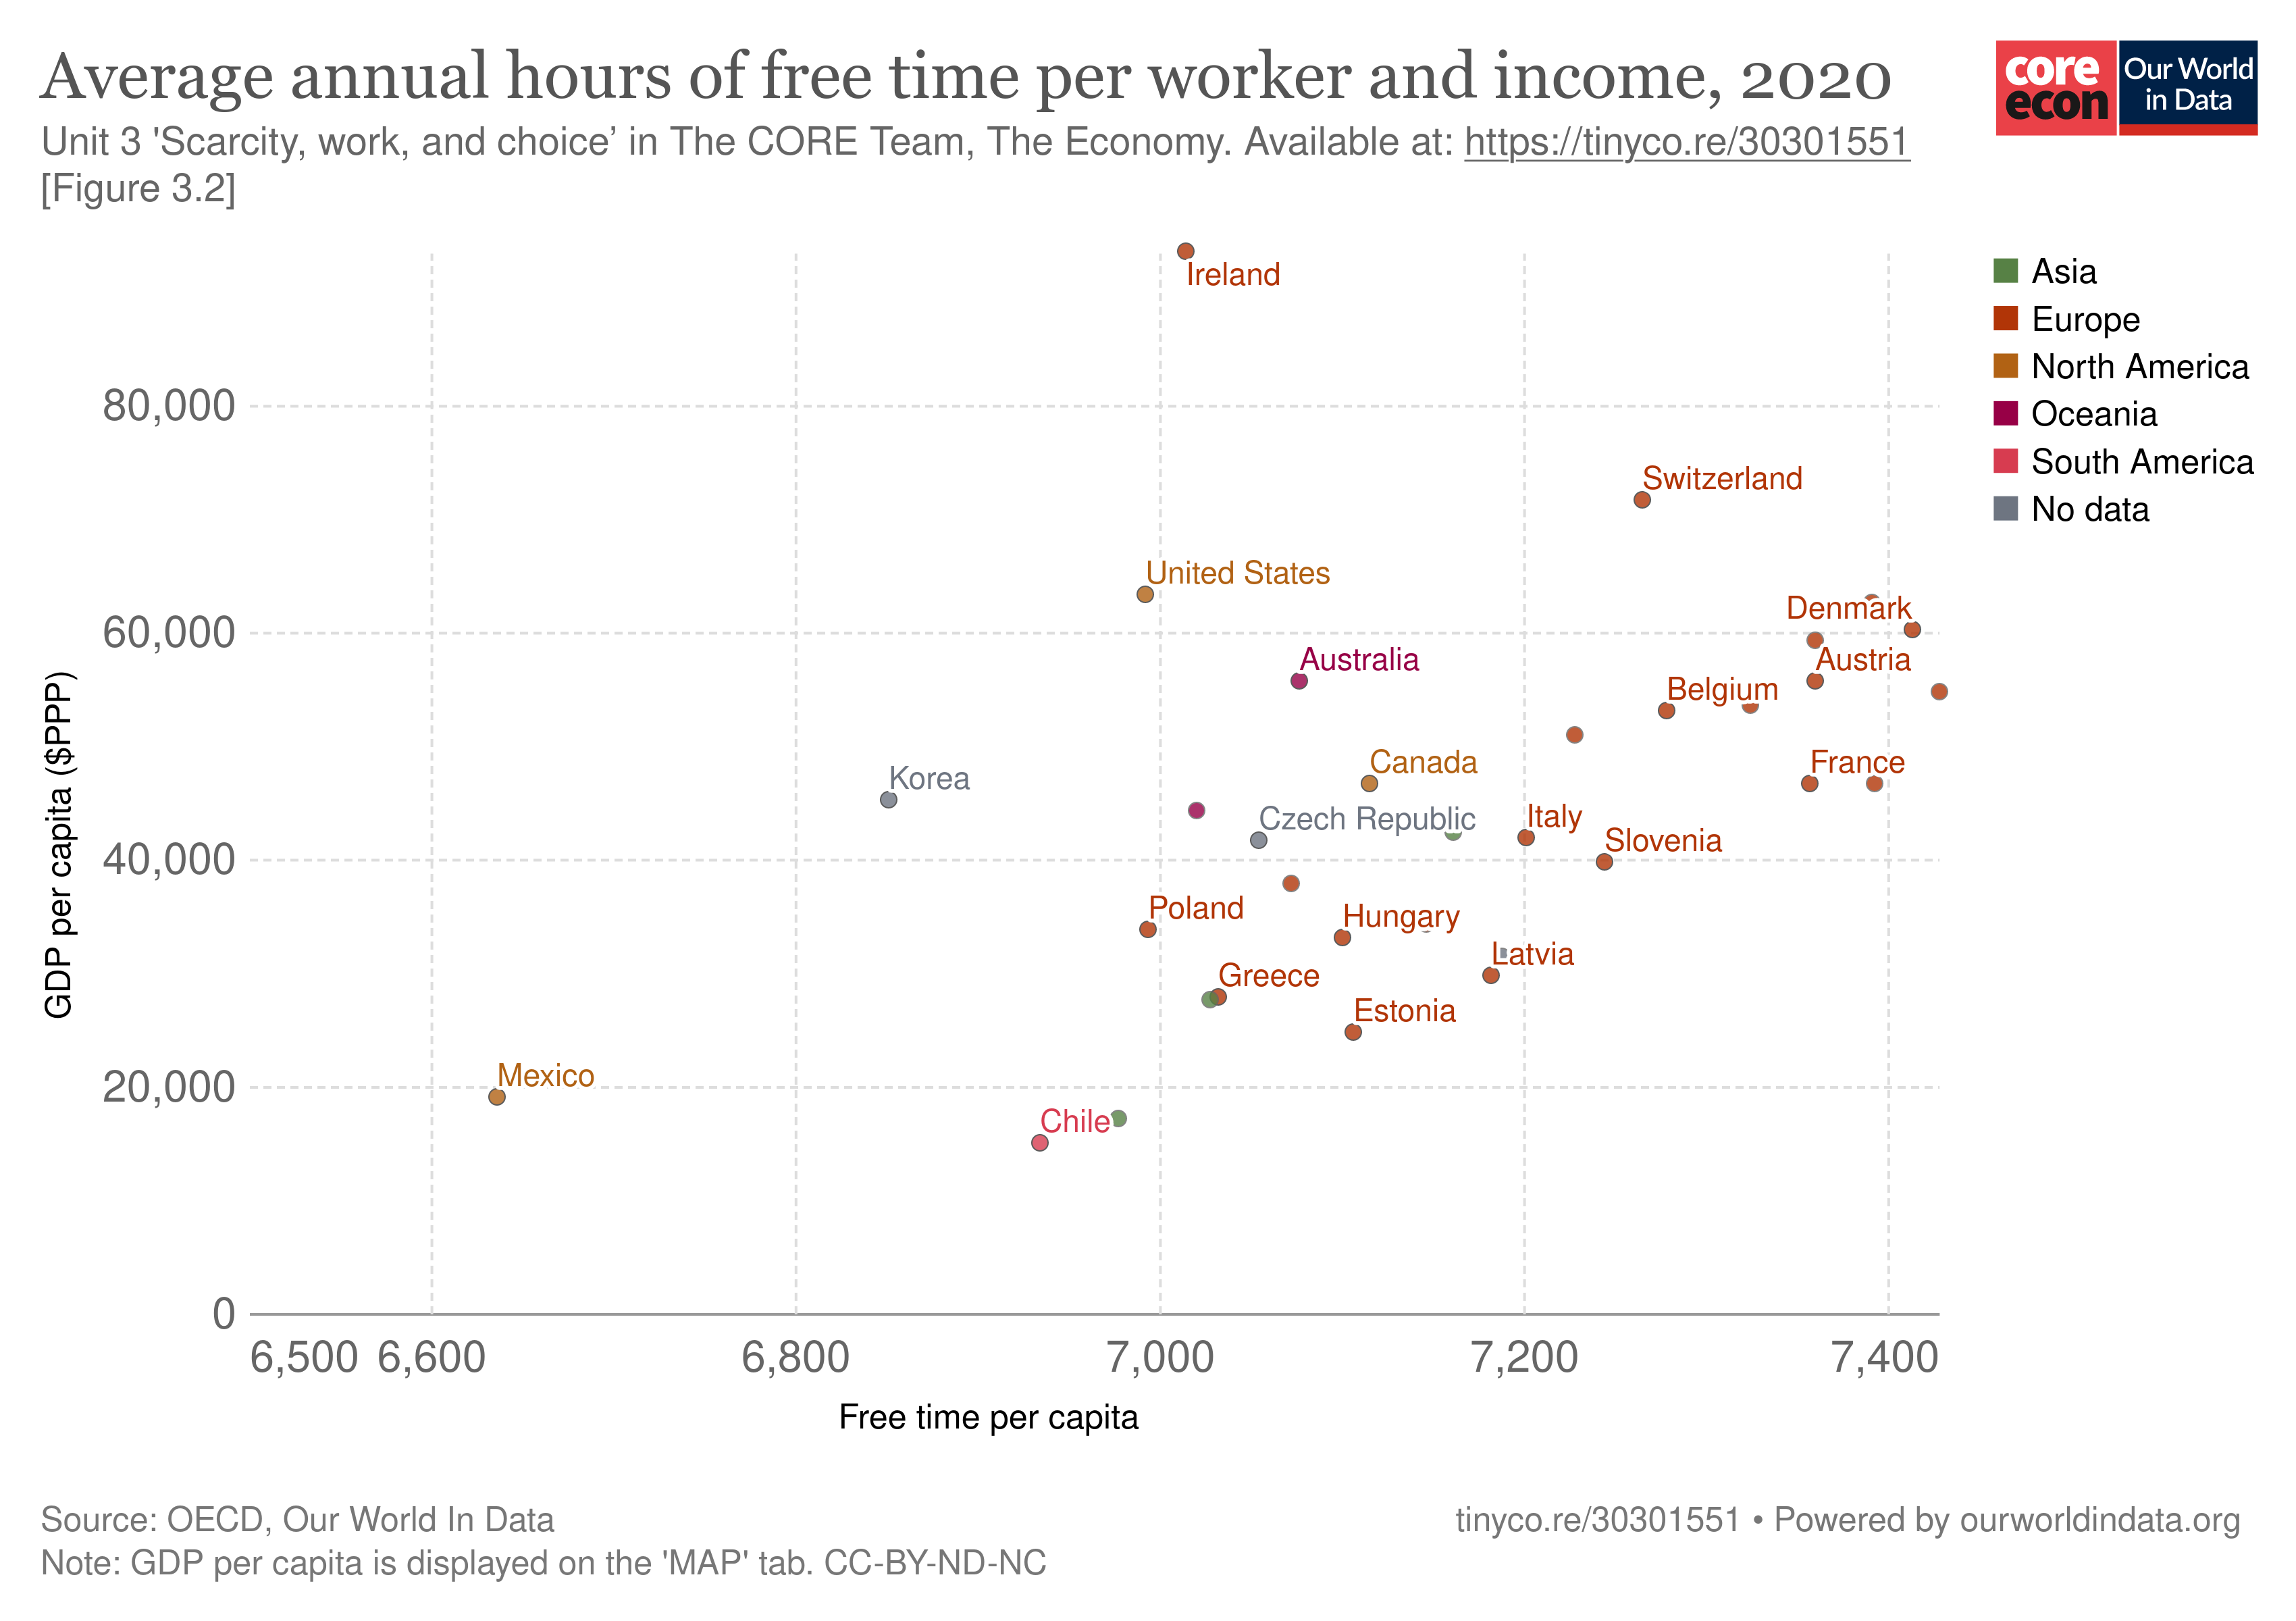
\includegraphics[width=\textwidth]{./figures/annual-hours-of-free-time-per-worker-and-income.png}
        \end{column}
        \begin{column}{0.5\textwidth}
            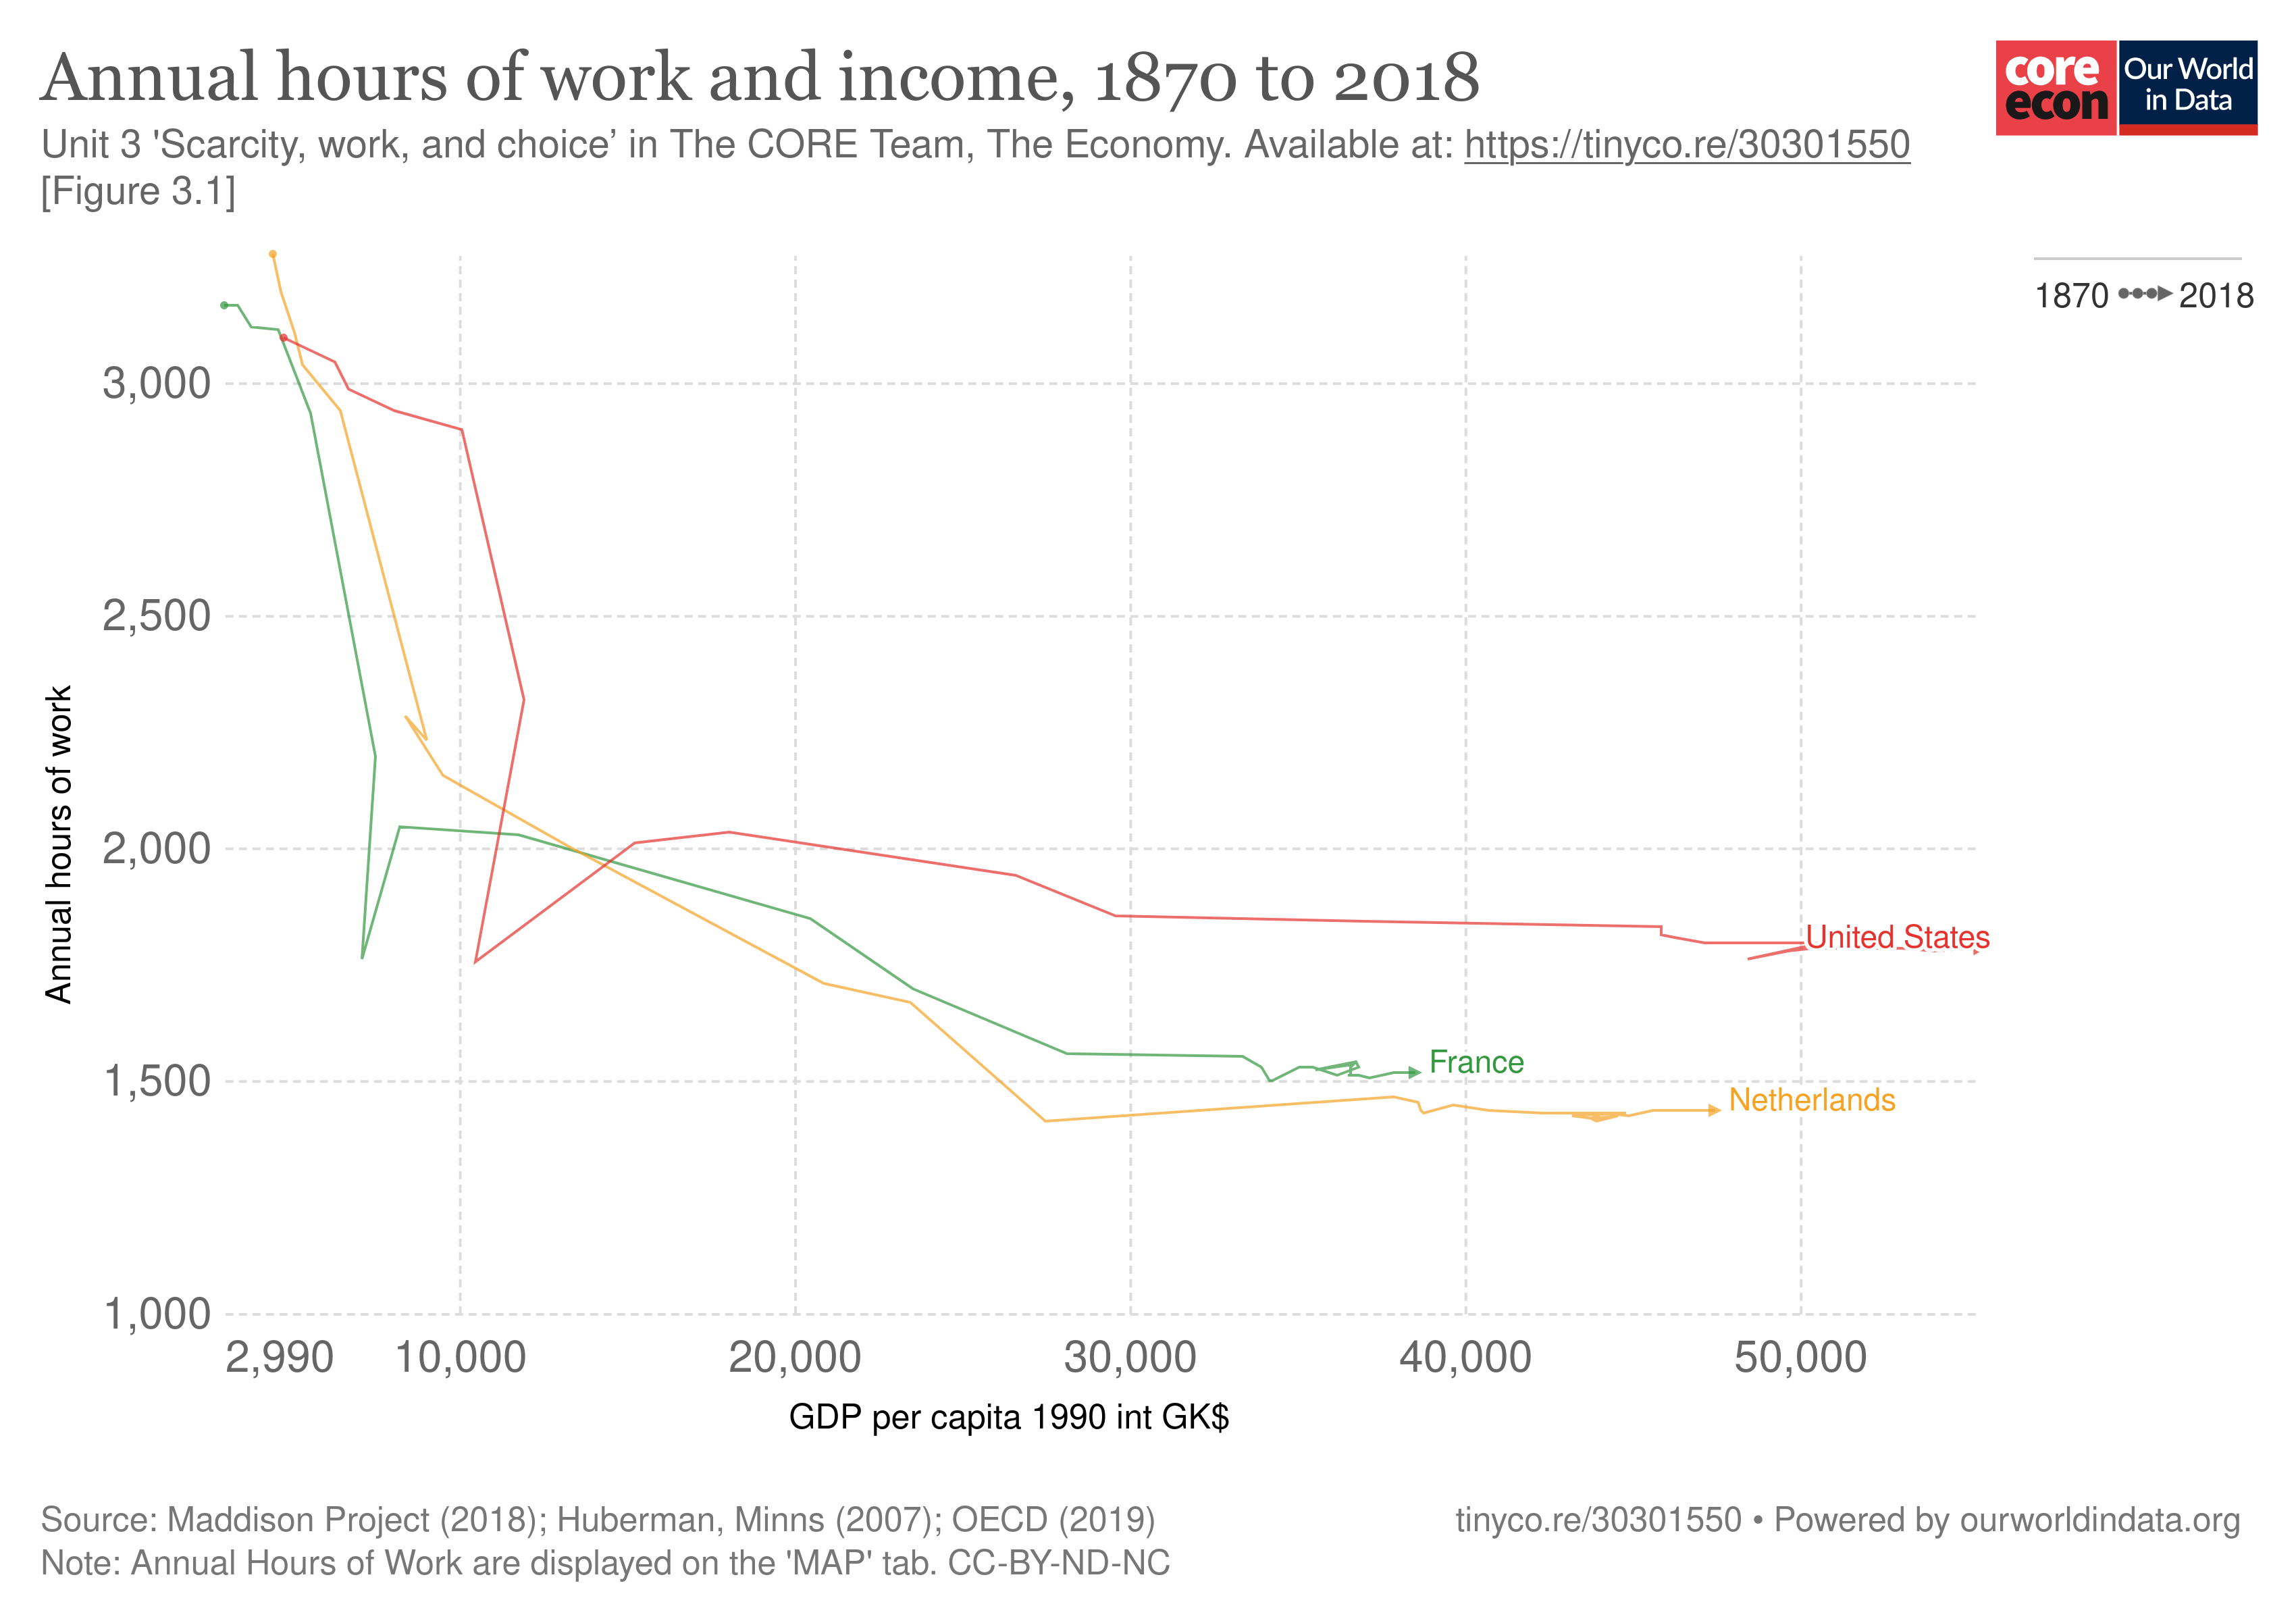
\includegraphics[width=\textwidth]{./figures/annual-hours-of-work-and-income-18702016.png}
        \end{column}
    \end{columns}

    \begin{itemize}
        \item Further reading: \url{https://tinyurl.com/4rhaepuk}
    \end{itemize}
\end{frame}


\section[Scarcity]{Scarcity and Choice}
\label{sec:Scarcity_and_Choice}

\begin{frame}[fragile]{Production Function for Study}
\label{slide:Production_Function}
    \only<1>{ Production function: how \alert{inputs} translate into \alert{output} }
    \only<2>{ \alert{Average product}: slope of the line connected with origin}
    \only<3>{ What if I want to know the average grade from 3hr to \alert{10}hr? }
    \only<4>{ What if I want to know the average grade from 3hr to \alert{6}hr? }
    \only<5>{ What if I want to know the average grade from 3hr to \alert{5}hr? }
    \only<6>{ What if I want to know the average grade from 3hr to \alert{4}hr? }
    \only<7>{ \scriptsize \alert{Marginal product}: ceteris paribus, change in output per \textbf{arbitrary small change} in input}
\begin{center}
\tiny
\begin{tabular}{c|c|c|c|c|c|c|c|c|c|c|c|c|c|c|c|c}
    Study hours  & 0  & 1  & 2  & 3  & 4  & 5  & 6  & 7  & 8  & 9  & 10  & 11  & 12  & 13  & 14  & 15$+$
    \\
    \hline
    Grade  & 0  & 20  & 33  & 42  & 50  & 57  & 63  & 69  & 74  & 78  & 81  & 84  & 86  & 88  & 89  & 90
    \\
\end{tabular}

\begin{tikzpicture}
  \datavisualization [scientific axes = clean,
                      % all axes = {grid},
                      x axis = {length = 10cm, label = {study hours}},
                      y axis = {length = 5cm, ticks = {many}, label = {grade}},
                      visualize as smooth line]
    % data [ headline = {x, y}, read from file = {grade.csv} ]
    data [ separator = \space, read from file = {grade.tab} ]
    info {
        \node[fill=red,circle,inner sep=1pt] (A) at ( visualization cs: x = 3, y = 42 ) {};
        \uncover<2> { \node[fill=black,circle,inner sep=1pt] (O) at ( visualization cs: x = 0, y = 0 ) {}; }
        \uncover<2> { \draw[-, blue, thick] (A) -- (O) ; }
        \uncover<3> { \node[fill=blue,circle,inner sep=1pt] (B) at ( visualization cs: x = 10, y = 81 ) {}; }
        \uncover<3> { \draw[shorten >=-1cm, shorten <=-1cm, thick, red] (A) -- (B); }
        \uncover<4> { \node[fill=blue,circle,inner sep=1pt] (C) at ( visualization cs: x = 6, y = 63 ) {}; }
        \uncover<4> { \draw[shorten >=-1cm, shorten <=-1cm, thick, red] (A) -- (C); }
        \uncover<5> { \node[fill=blue,circle,inner sep=1pt] (D) at ( visualization cs: x = 5, y = 57 ) {}; }
        \uncover<5> { \draw[shorten >=-1cm, shorten <=-1cm, thick, red] (A) -- (D); }
        \uncover<6> { \node[fill=blue,circle,inner sep=1pt] (E) at ( visualization cs: x = 4, y = 50 ) {}; }
        \uncover<6> { \draw[shorten >=-1cm, shorten <=-1cm, thick, red] (A) -- (E); }
        \uncover<7> { \node (F) at ( visualization cs: x = 4, y = 50 ) {}; }
        \uncover<7> { \draw[shorten >=-1cm, shorten <=-1cm, thick, red] (A) -- (F); }
    };
\end{tikzpicture}
\end{center}
\end{frame}

\begin{frame}[fragile]{Diminishing Marginal Product of Study}
\label{slide:Diminishing_Marginal_Product_of_Study}

Study become less productive the more you study! $ \Rightarrow  $ Scarcity in nature

\begin{center}
\tiny
\begin{tabular}{c|c|c|c|c|c|c|c|c|c|c|c|c|c|c|c|c}
    Study hours  & 0  & 1  & 2  & 3  & 4  & 5  & 6  & 7  & 8  & 9  & 10  & 11  & 12  & 13  & 14  & 15$+$
    \\
    \hline
    Grade  & 0  & 20  & 33  & 42  & 50  & 57  & 63  & 69  & 74  & 78  & 81  & 84  & 86  & 88  & 89  & 90
    \\
    \hline
    mar. grade  & 20  & 13  & 9  & 8  & 7  & 6  & 6  & 5  & 4  & 3  & 3  & 2  & 2  & 1  &  1 & 0
    \\
\end{tabular}

\begin{tikzpicture}
  \datavisualization [scientific axes = clean,
                      % all axes = {grid},
                      x axis = {length = 10cm, label = {study hours}},
                      y axis = {length = 5cm, ticks = {many}, label = {marginal grade}},
                      visualize as smooth line]
    % data [ headline = {x, y}, read from file = {MP.csv} ];
    data [ separator = \space, read from file = {MP.tab} ];
\end{tikzpicture}
\end{center}

\end{frame}

\begin{frame}{The Production Possibility Frontier}
\label{slide:The_Production_Possibility_Frontier}

\only<1> { Do you want to study all day? Probably not! }
\only<2> { \small \textbf{Supply side} trade off between free time and grade $ \Rightarrow  $ M{\tiny arginal} R{\tiny ate of }T{\tiny ransformation}}

\begin{center}
\tiny
\begin{tabular}{c|c|c|c|c|c|c|c|c|c|c|c|c|c|c|c|c}
    Study hours  & 0  & 1  & 2  & 3  & 4  & 5  & 6  & 7  & 8  & 9  & 10  & 11  & 12  & 13  & 14  & 15$+$
    \\
    \hline
    Free time & 24  & 23  & 22  & 21  & 20  & 19  & 18  & 17  & 16  & 15  & 14  & 13  & 12  & 11  & 10  & 9$-$
    \\
    \hline
    Grade  & 0  & 20  & 33  & 42  & 50  & 57  & 63  & 69  & 74  & 78  & 81  & 84  & 86  & 88  & 89  & 90
    \\
    \hline
    MRT ($=$MP) & 20  & 13  & 9  & 8  & 7  & 6  & 6  & 5  & 4  & 3  & 3  & 2  & 2  & 1  &  1 & 0
    \\
\end{tabular}

\begin{tikzpicture}
  \datavisualization [scientific axes = clean,
                      % all axes = {grid},
                      x axis = {length = 10cm, label = {Free time}},
                      y axis = {length = 5cm, ticks = {many}, label = {grade}},
                      visualize as smooth line]
    % data [ headline = {x, y}, read from file = {PPF.csv} ];
    data [ separator = \space, read from file = {PPF.tab} ]
    info {
        \uncover<2> { \node[fill=red,circle,inner sep=1pt] (A) at ( visualization cs: x = 21, y = 42 ) {}; }
        \uncover<2> { \node (B) at ( visualization cs: x = 22, y = 33 ) {}; }
        \uncover<2> { \draw[shorten >=-1cm, shorten <=-1cm, thick, red] (A) -- (B); }
    };
\end{tikzpicture}
\end{center}

\end{frame}

\begin{frame}[fragile]{Utility Function}
\label{slide:Utility_Function}
    \begin{itemize}
        \item As a student you \alert{value} two things: \alert{free time} and \alert{grade}
        \item However, higher grade $ \Rightarrow  $ sacrifice your free time!
        % \item So on figure there are totally three things: free time, grade and happiness
    \end{itemize}

    \begin{center}

        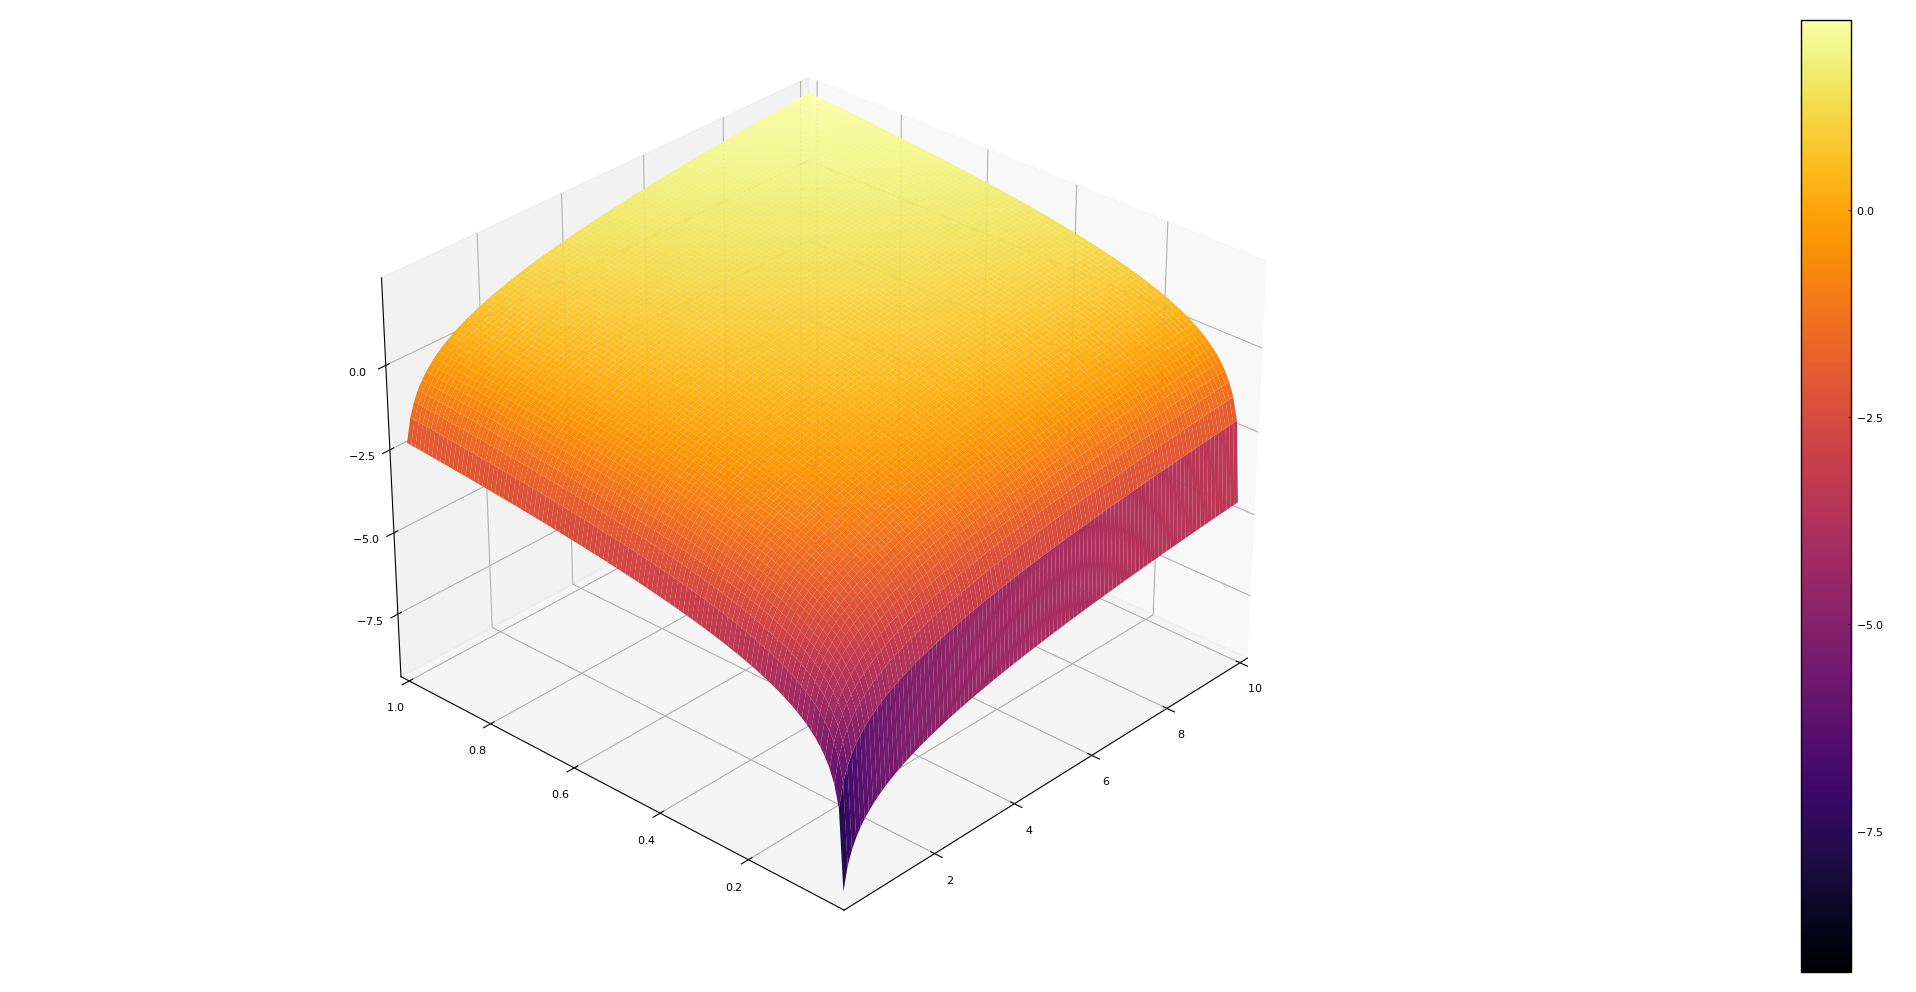
\includegraphics[width=\textwidth]{./figures/utility.png}
        % \begin{tikzpicture}
        %     \begin{axis}[xmax=10,ymax=4, xmin=0, ymin=0]
        %         \addplot3[mesh, samples = 50]{ln(x) + ln(y)}
        %     \end{axis}
        % \end{tikzpicture}
    \end{center}

\end{frame}

\begin{frame}{Visualizing 3-D Function on 2-D plane}
\label{slide:Visualizing_3_D_Function_on_2_D_plane}

    \begin{itemize}
        \item It is hard for me to process 3D figure \faFrownO...  What should I do?
        \item \textbf{Contours}:``standing'' at the peak and look down
        \begin{itemize}
            \item e.g. \alert{\href{https://www.alltrails.com/}{map on Alltrails}}
        \end{itemize}
    \end{itemize}

    \begin{center}
        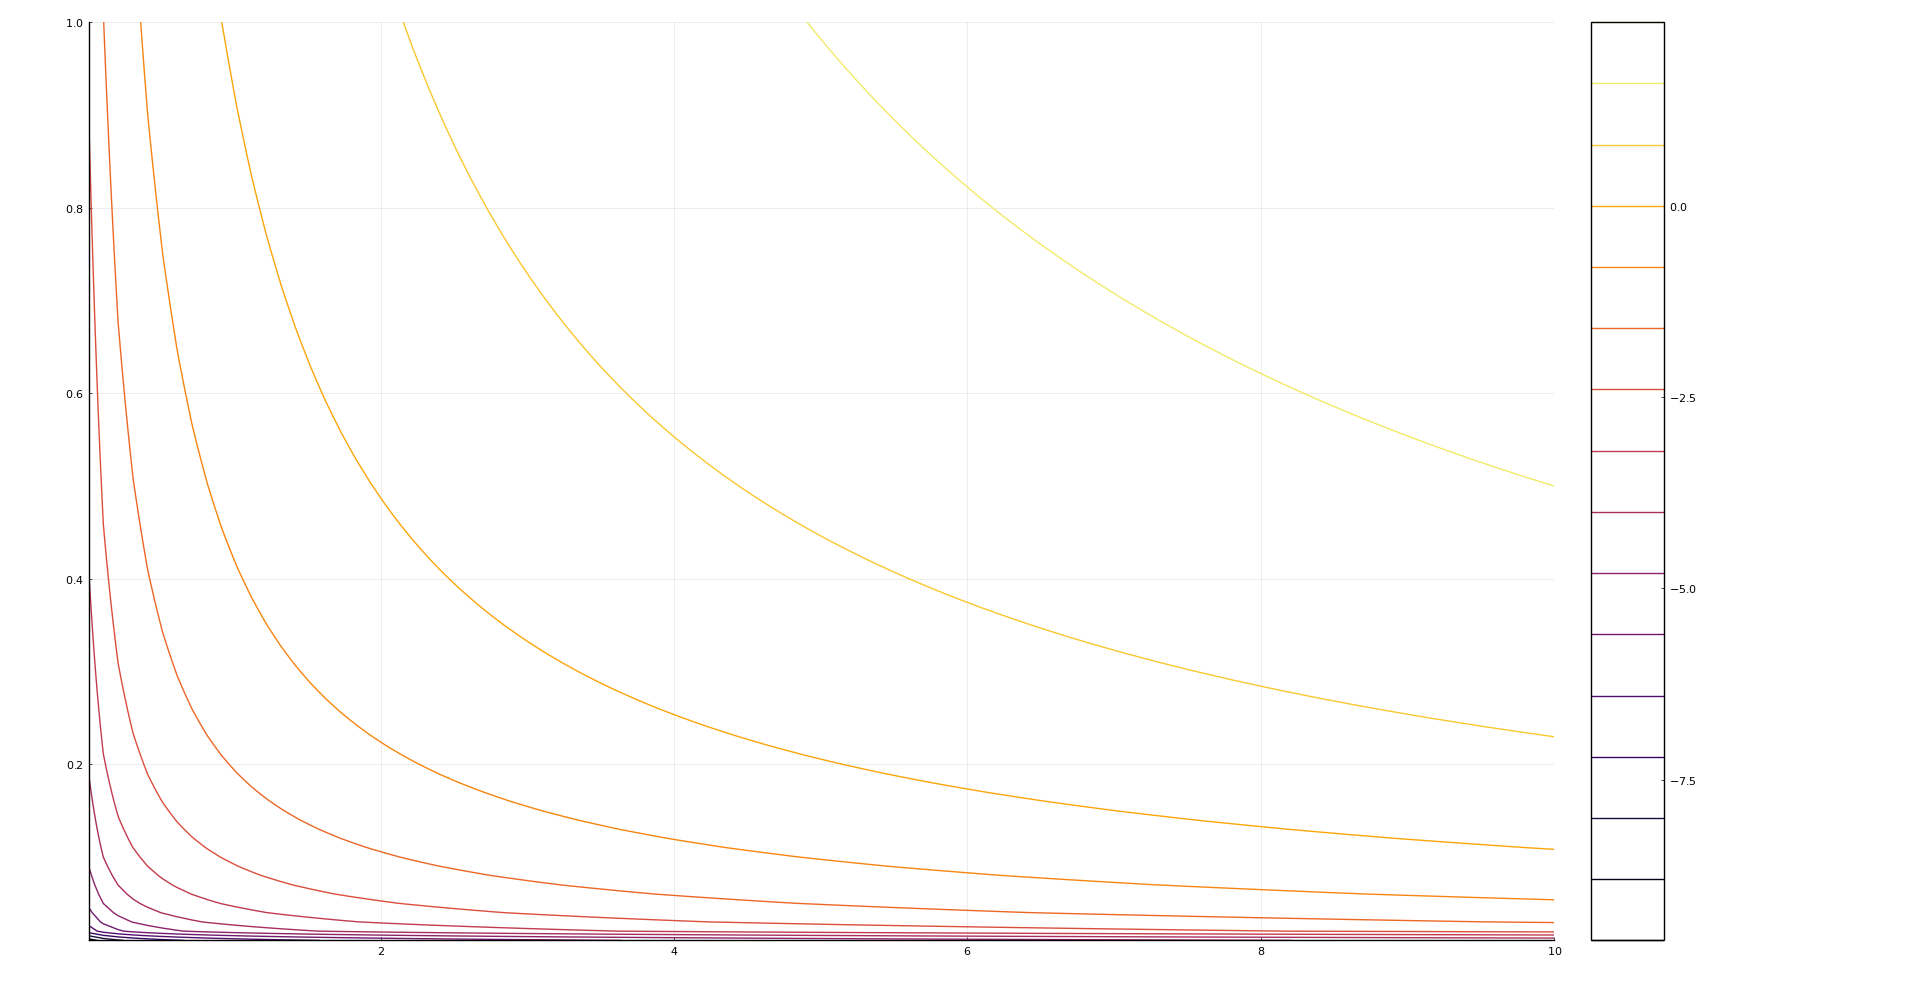
\includegraphics[width=\textwidth]{./figures/utility_contour.png}
    \end{center}

\end{frame}

\begin{frame}{Indifference Curve}
\label{slide:Indifference_Curve}

The contour figure on utility function is indifference curve!

\begin{columns}
    \begin{column}{0.4\textwidth}
        \begin{itemize}
            \item \textbf{Def}: Combination of goods that gives \alert{same level} of utility
            \item M{\tiny arginal }R{\tiny ate of }S{\tiny ubstitution}: \textbf{Demand side} trade off between free time and grade
            \begin{itemize}
                \item Graphical representation is the tangent line on indifference curve, similar to MRT
            \end{itemize}
        \end{itemize}
    \end{column}
    \begin{column}{0.6\textwidth}
        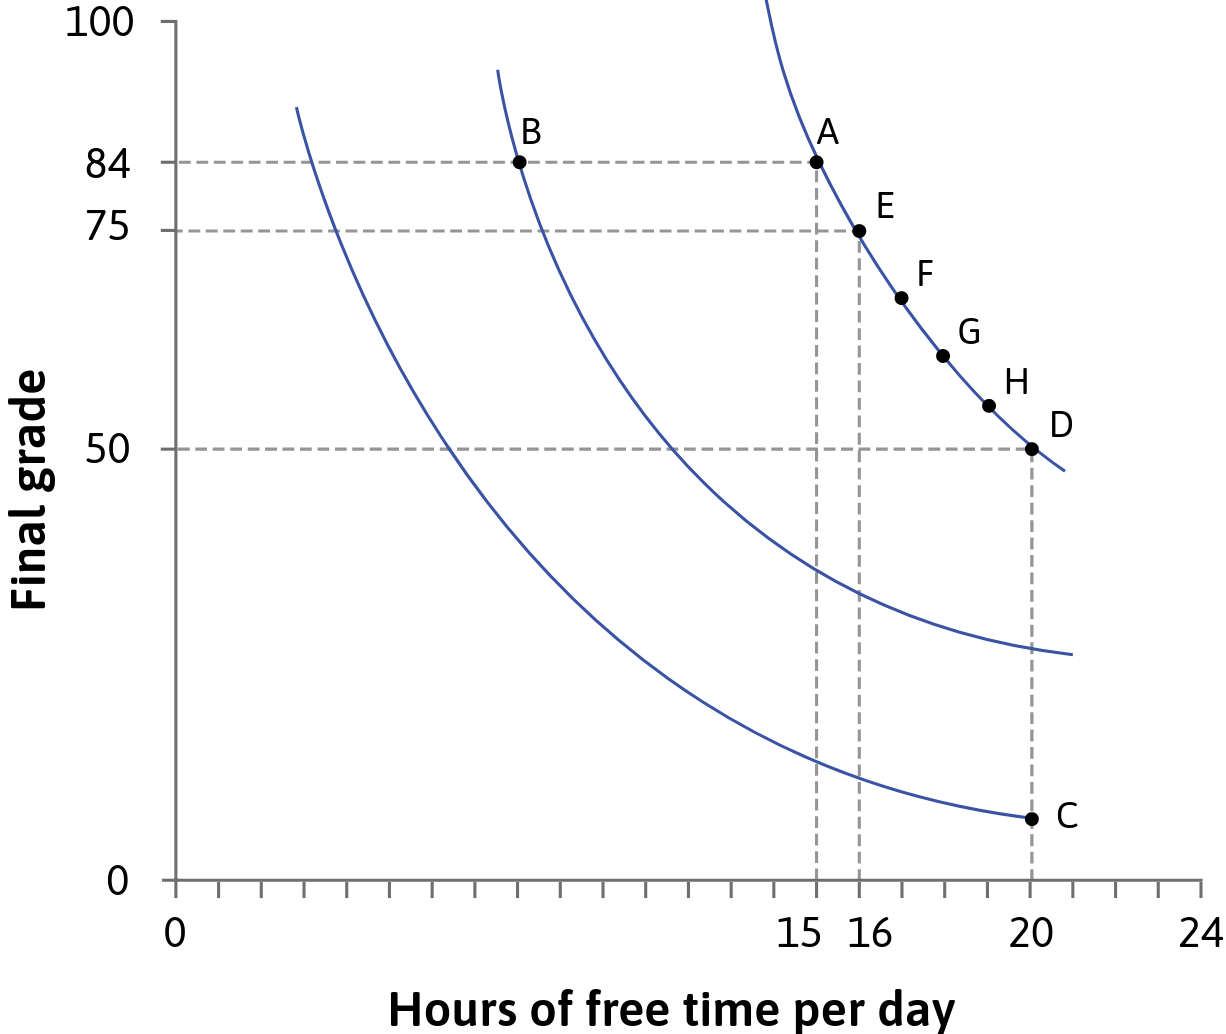
\includegraphics[width=\textwidth]{./figures/IndiffCurve.png}
    \end{column}
\end{columns}

\end{frame}

\section[Decision]{Decision-making under Scarcity}
\label{sec:Decision_making_under_Scarcity}

\begin{frame}{Optimal Social Resource Distrbution}
\label{slide:Constrained_Choice_Problem}
    \small
    In the grade example, you are both the \alert{consumer} and \alert{producer} of grade and free time
    \begin{columns}
        \begin{column}{0.5\textwidth}
            \begin{itemize}
                \item What you as a \alert{social planner} want to do is to accord the \alert{demand side} trade off in \textbf{MRS} with the \alert{supply side} trade in \textbf{MRT}
                \item Recall that on the figure, both MRS and MRT are \alert{tangent lines}, and thus the \alert{optimal social resource distribution} must allow utility function and production possibility frontier \textbf{tangent at the same point}!
            \end{itemize}
        \end{column}
        \begin{column}{0.5\textwidth}
            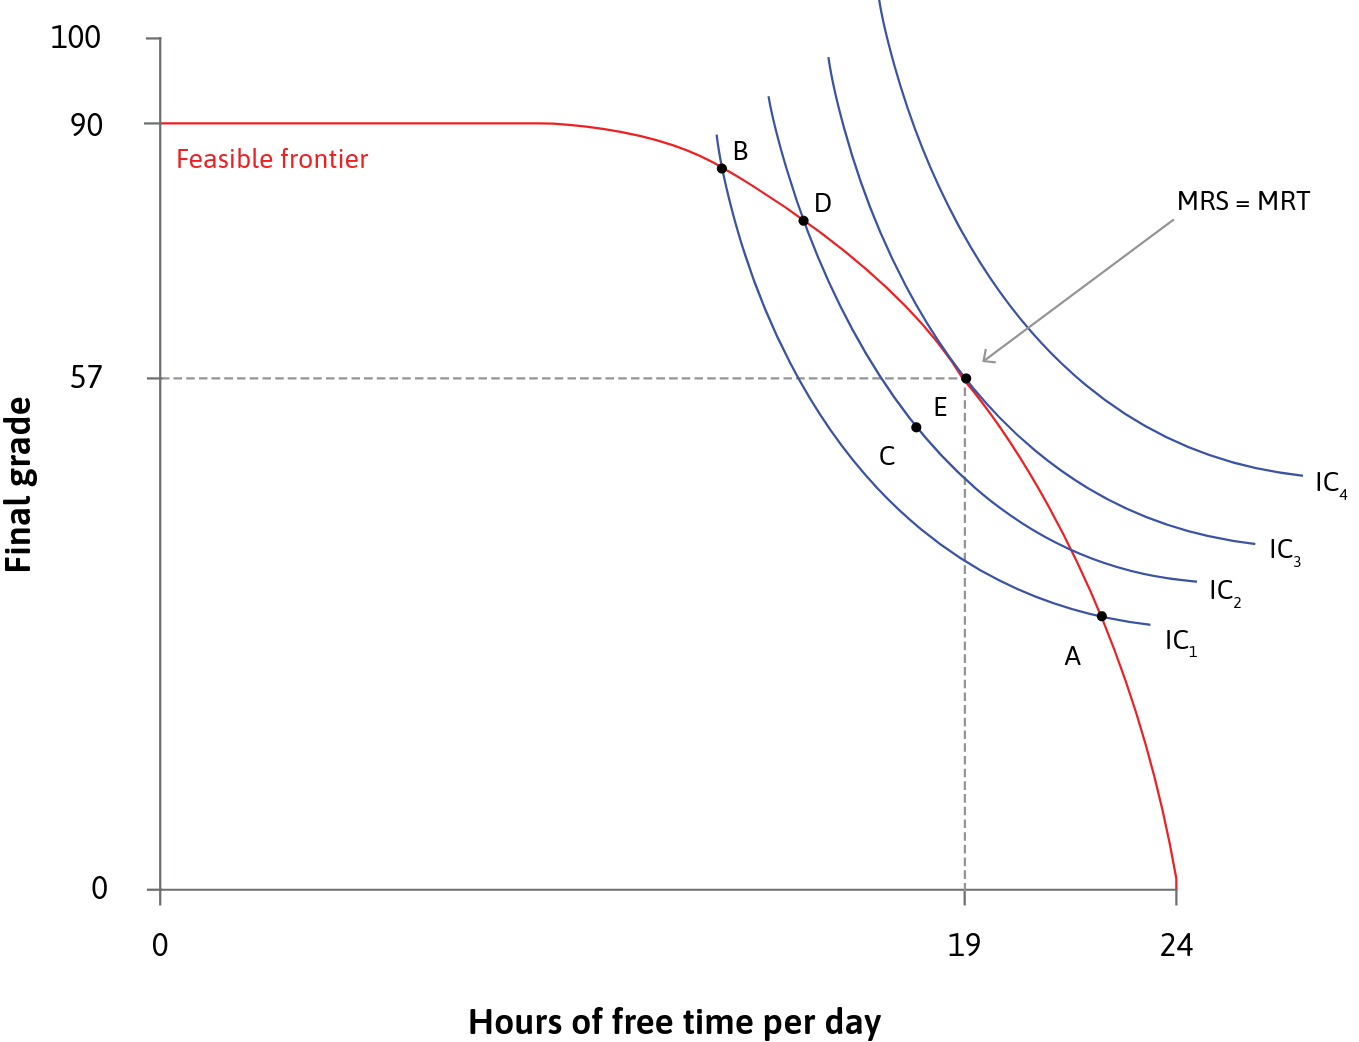
\includegraphics[width=\textwidth]{./figures/MRSMRT.png}
        \end{column}
    \end{columns}

\end{frame}

\begin{frame}{Prices \& Market Structure}
\label{slide:Prices}
    \begin{itemize}
        \item What real world things make $ MRT = MRS $? $ \Rightarrow  $ Prices!
        \item \textbf{Competitive} price determines the market trade off between two goods
        \begin{tabular}{c|c|c|c|c}
            market
                & labor & credit & bond & capital
            \\
            \hline
            price
                & wage & interest rate & bond price & rental / purchase price
            \\
        \end{tabular}
        \item Prices are not necessary be competitive $ \Rightarrow  $ \alert{market structure}
        \begin{itemize}
            \item Perfect competition
            \item Monopolistic competition
            \item Monopoly
            \item Oligopoly
        \end{itemize}

    \end{itemize}
\end{frame}

\begin{frame}{Better Technology}
\label{slide:Optimal_Decision_Making}
    \begin{center}
        What happens when the feasible frontier changes?
    \end{center}

    \begin{itemize}
        \item PPF expands \alert{only on grain production} $ \Rightarrow  $ why?
        \item Better tech $ \Rightarrow  $ more grain production and more free time!
    \end{itemize}

    \begin{center}
        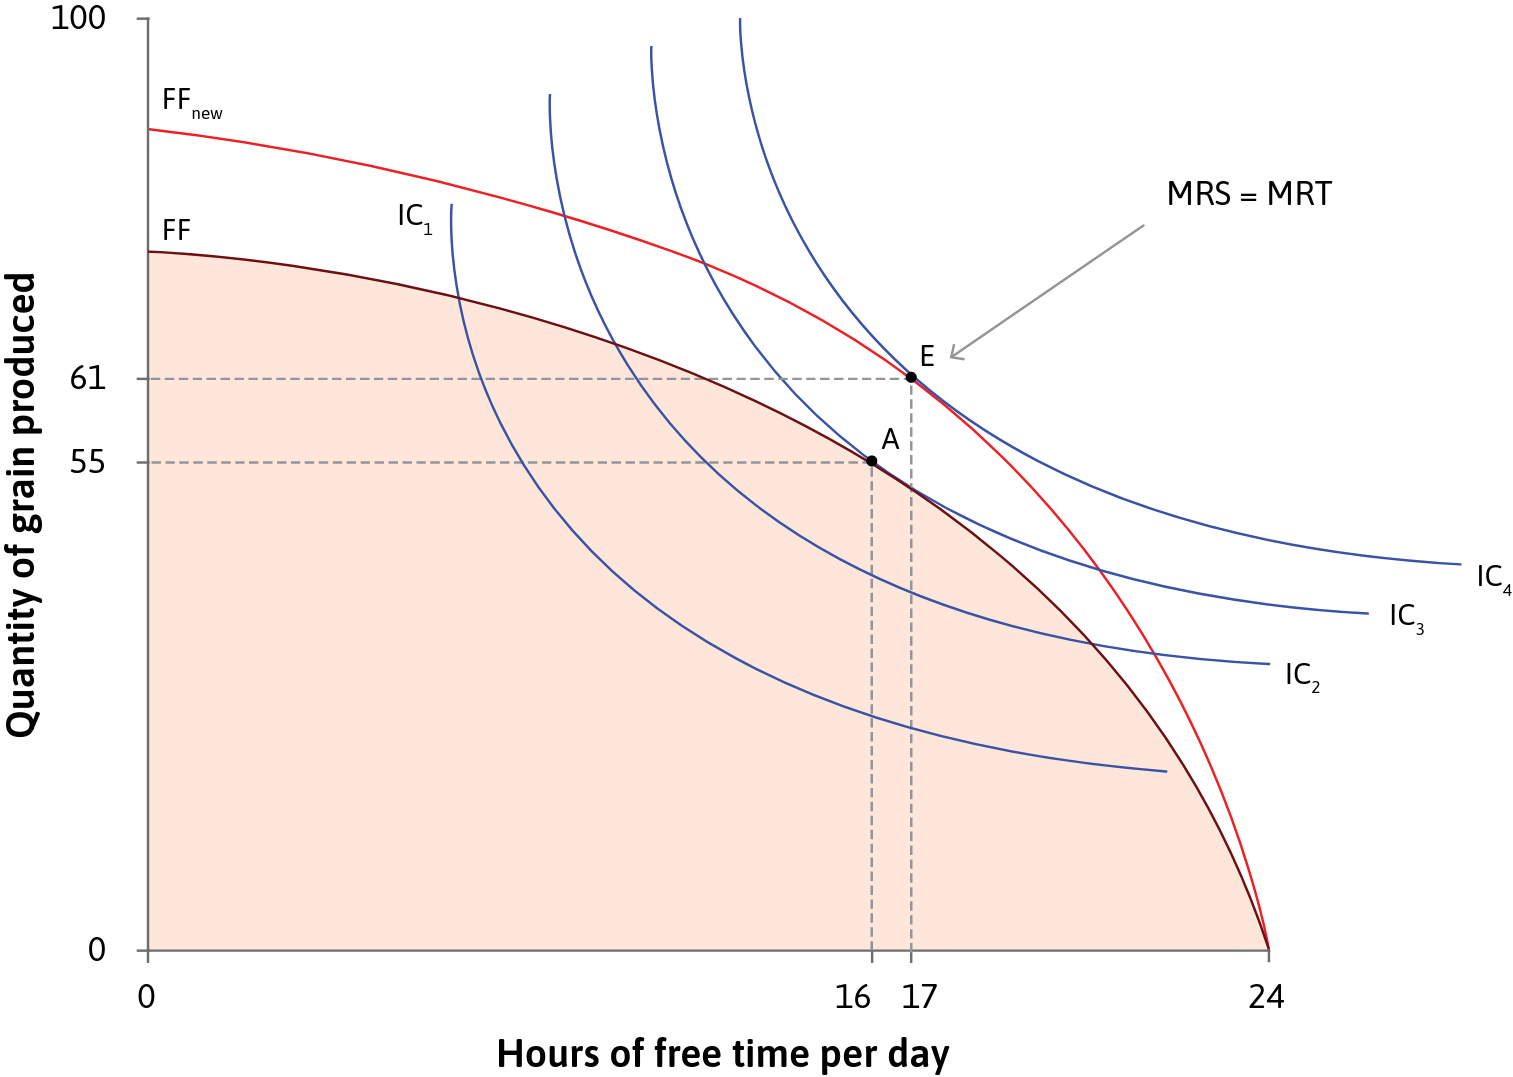
\includegraphics[width=0.65\textwidth]{./figures/OptimalChange.png}
    \end{center}
\end{frame}

\section[I\&SEffect]{Income and Substitution Effects}
\label{sec:Income_and_Substitution_Effects}

\begin{frame}[fragile]{Working Hours}
\label{slide:Working_Hours}
Budget constraint is $ c = w \times (24 - t) $, represented by the triangle area
    \begin{center}
        \scriptsize
        \begin{tabular}{c|c|c|c|c|c|c|c|c|c}
            Hours of work   &  0   &  2   &  4   &  6   &  8   &  10   &  12   &  14   &  16
            \\
            \hline
            Free time, $t$   &  24   &  22   &  20   &  18   &  16   &  14   &  12   &  10   &  8
            \\
            \hline
            Consumption, $c$   &  0   &  \$30   &  \$60   &  \$90   &  \$120   &  \$150   &  \$180   &  \$210   &  \$240
            \\
        \end{tabular}
    \end{center}

    % \begin{center}
    %     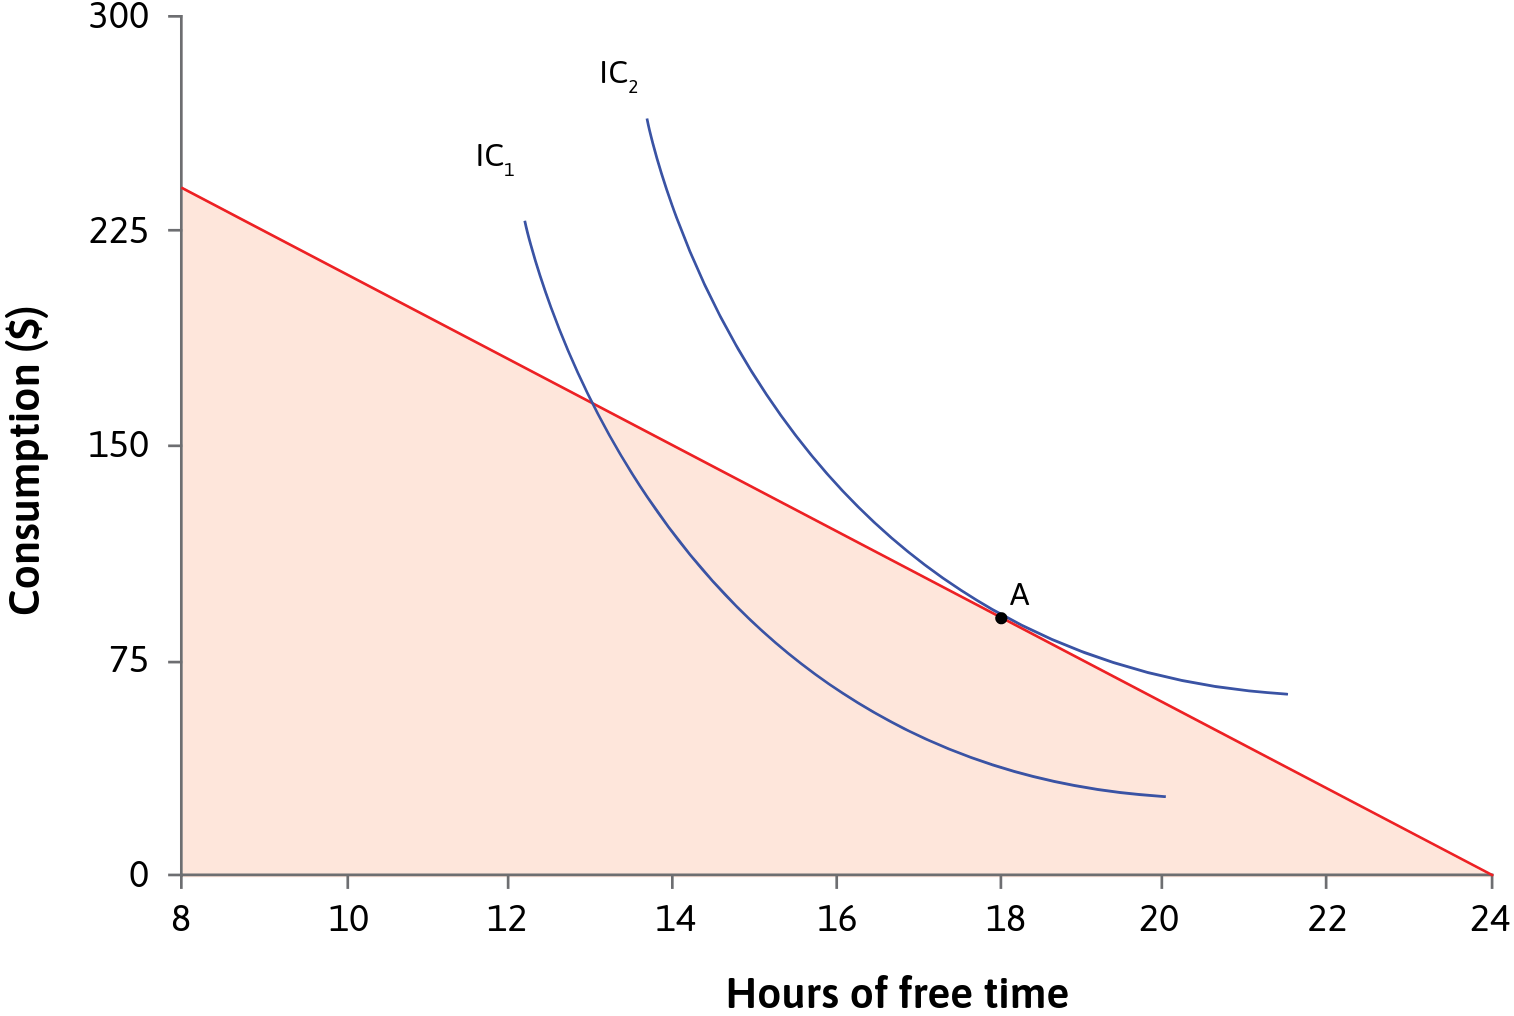
\includegraphics[width=0.65\textwidth]{./figures/DecisionMaking.png}
    % \end{center}

    % \begin{center}
    %     \begin{tikzpicture}
    %         \begin{axis}[sciclean, height = 5cm, try min ticks=5]
    %             \addplot[color = red, dashed, samples = 50]{x^2};
    %         \end{axis}
    %     \end{tikzpicture}
    % \end{center}


    \begin{center}
        \begin{tikzpicture}
            \datavisualization [scientific axes = clean,
                              x axis = {length = 8cm, label = {Free time}},
                              y axis = {length = 4cm, ticks = {few}, label = {grain}},
                              visualize as smooth line/.list={lowwage, highwage},
                              style sheet = vary dashing,
                              legend = north east inside,
                              lowwage = {label in legend = {text = low wage}},
                              highwage = {label in legend = {text = high wage}}
            ]
              data [set=lowwage, format=function] {
                var x : interval [8:24];
                func y = 15 * (24 - \value x);
              }
              data [set=highwage, format=function] {
                var x : interval [8:24];
                func y = 25 * (24 - \value x);
              }
              info {
                \node (A) at ( visualization cs: x = 17.5, y = 120 ) {};
                \node (B) at ( visualization cs: x = 12.5, y = 250 ) {};
                \draw[thick, blue, name path = AB] (A) to[bend left=30]
                    node[pos=0.35,draw,fill=red,circle,inner sep=1pt, left] (a) {}
                    (B);
                \node[xshift = 1cm, yshift = 0.4cm, at = (A)] (C){};
                \node[xshift = 1cm, yshift = 0.4cm, at = (B)] (D){};
                \draw[thin, orange, name path = CD]
                    (C) to[bend left=30]
                    node[pos=0.5,draw,fill=red,circle,inner sep=1pt] (b) {}
                    (D);
              }
            ;
        \end{tikzpicture}
    \end{center}


\end{frame}

\begin{frame}[fragile]{Working Hours}
\label{slide:Working_Hours}
Budget constraint is $ c = w \times (24 - t) $, represented by the triangle area
    \begin{center}
        \scriptsize
        \begin{tabular}{c|c|c|c|c|c|c|c|c|c}
            Hours of work   &  0   &  2   &  4   &  6   &  8   &  10   &  12   &  14   &  16
            \\
            \hline
            Free time, $t$   &  24   &  22   &  20   &  18   &  16   &  14   &  12   &  10   &  8
            \\
            \hline
            Consumption, $c$   &  0   &  \$30   &  \$60   &  \$90   &  \$120   &  \$150   &  \$180   &  \$210   &  \$240
            \\
        \end{tabular}
    \end{center}

    \begin{center}
        \begin{tikzpicture}
            \datavisualization [scientific axes = clean,
                              x axis = {length = 8cm, label = {Free time}},
                              y axis = {length = 4cm, ticks = {few}, label = {grain}},
                              visualize as smooth line/.list={lowwage, highwage},
                              style sheet = vary dashing,
                              legend = north east inside,
                              lowwage = {label in legend = {text = low wage}}
                              % highwage = {label in legend = {text = high wage}}
            ]
              data [set=lowwage, format=function] {
                var x : interval [8:24];
                func y = 15 * (24 - \value x);
              }
              % data [set=highwage, format=function] {
              %   var x : interval [8:24];
              %   func y = 25 * (24 - \value x);
              % }
              info {
                \node (A) at ( visualization cs: x = 17.5, y = 115 ) {};
                \node (B) at ( visualization cs: x = 12.5, y = 200 ) {};
                \draw[thick, blue, name path = AB] (A) to[bend left=20]
                    node[pos=0.4,draw,fill=red,circle,inner sep=1pt, left] (a) {}
                    (B);
                \node[xshift = -1cm, yshift = -1cm, at = (A)] (C){};
                \node[xshift = -1cm, yshift = -1cm, at = (B)] (D){};
                \draw[thin, orange, name path = CD]
                    (C) to[bend left=20]
                    % node[pos=0.5,draw,fill=red,circle,inner sep=1pt] (b) {}
                    (D);
              }
            ;
        \end{tikzpicture}
    \end{center}

    % \begin{center}
    %     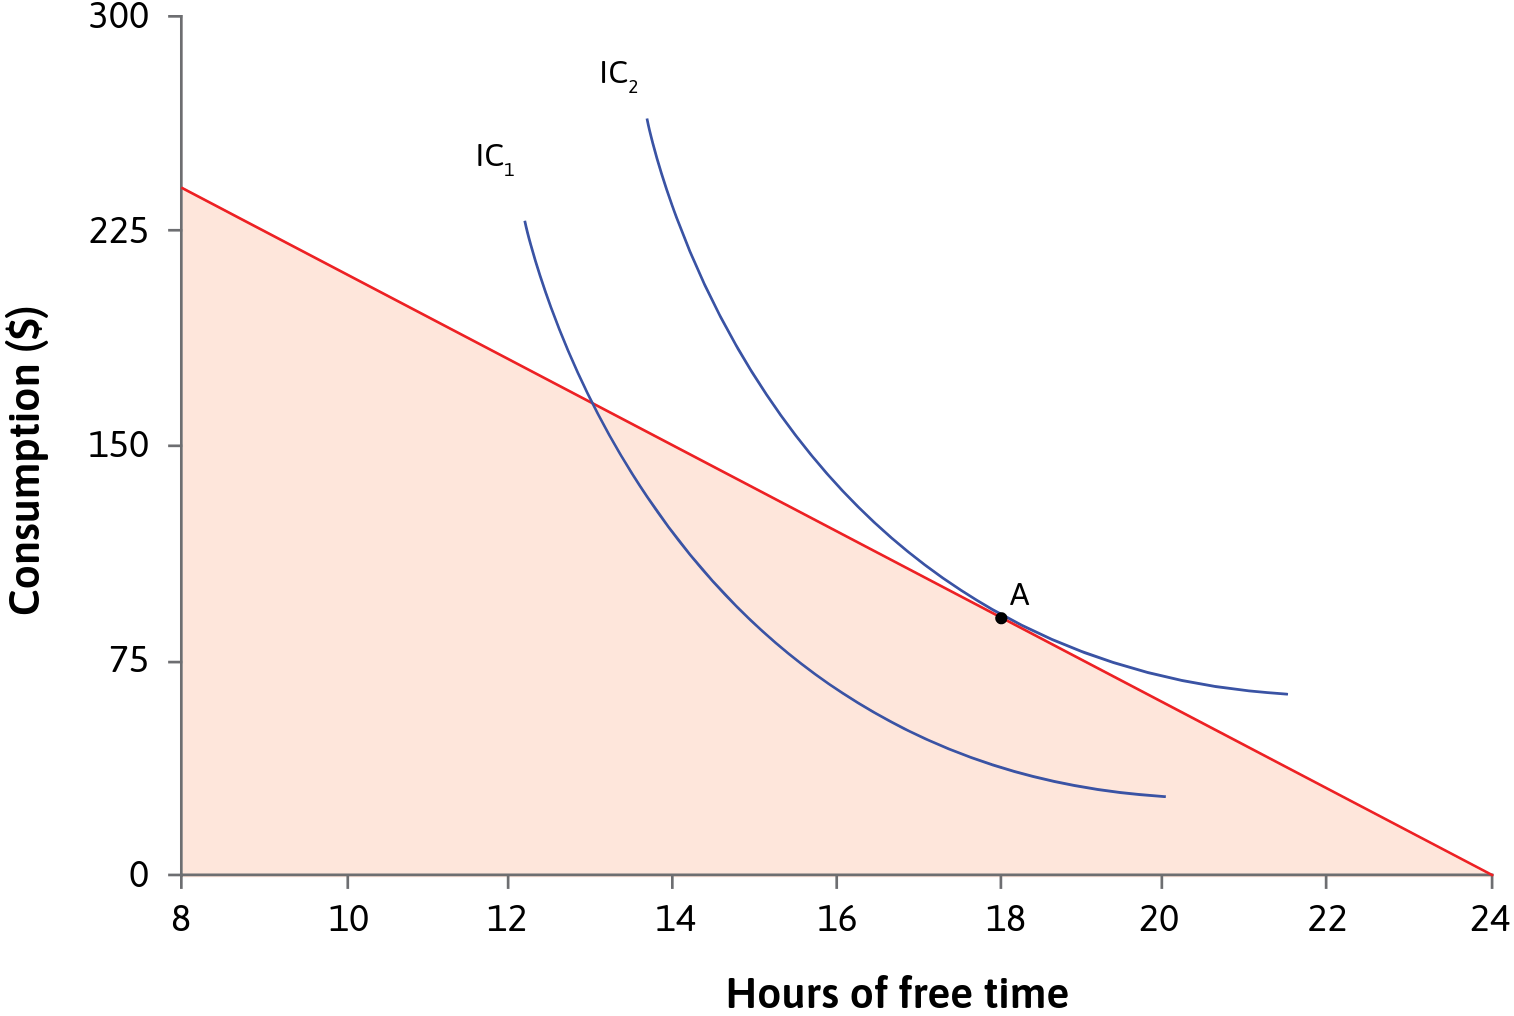
\includegraphics[width=0.65\textwidth]{./figures/DecisionMaking.png}
    % \end{center}

    % \begin{center}
    %     \begin{tikzpicture}
    %         \begin{axis}[sciclean, height = 5cm, try min ticks=5]
    %             \addplot[color = red, dashed, samples = 50]{x^2};
    %         \end{axis}
    %     \end{tikzpicture}
    % \end{center}

\end{frame}

\begin{frame}{Two Important Effects}
\label{slide:Two_Important_Effects}
    Wage change will affect the slope of budget constraint.

    A wage increase will have two effects:
    \begin{enumerate}
        \item \textbf{Income effect}: Total earnings $ \uparrow  $, if you work the same hour
        \begin{itemize}
            \item \alert{parallel shift} of the budget constraint
        \end{itemize}

        \item \textbf{Substitution effect}: the opportunity cost of leisure is higher
        \begin{itemize}
            \item \alert{rotation} of the budget constraint
        \end{itemize}
    \end{enumerate}
\end{frame}


\begin{frame}[fragile]{Income Effect}
\label{slide:Working_Hours}

Both free time and grain $ \uparrow  $ $ \Rightarrow  $ Both goods are \alert{normal goods}

    \begin{center}
        \begin{tikzpicture}
            \datavisualization [scientific axes = clean,
                              x axis = {length = 8cm, label = {Free time}},
                              y axis = {length = 4cm, ticks = {few}, label = {grain}},
                              visualize as smooth line/.list={lowwage, highwage},
                              style sheet = vary dashing,
                              legend = north east inside,
                              lowwage = {label in legend = {text = low wage}},
                              highwage = {label in legend = {text = high wage}}
            ]
              data [set=lowwage, format=function] {
                var x : interval [8:24];
                func y = 15 * (24 - \value x);
              }
              data [set=highwage, format=function] {
                var x : interval [8:24];
                func y = 20 * 24 - 15 * \value x;
              }
              info {
                \node (A) at ( visualization cs: x = 17.5, y = 120 ) {};
                \node (B) at ( visualization cs: x = 12.5, y = 250 ) {};
                \draw[thick, blue, name path = AB] (A) to[bend left=32]
                    node[pos=0.35,draw,fill=red,circle,inner sep=1pt, left] (a) {}
                    (B);
                \node[xshift = 1.1cm, yshift = 1cm, at = (A)] (C){};
                \node[xshift = 1.1cm, yshift = 1cm, at = (B)] (D){};
                \draw[thin, orange, name path = CD]
                    (C) to[bend left=32]
                    node[pos=0.35,draw,fill=red,circle,inner sep=1pt] (b) {}
                    (D);
              }
            ;
        \end{tikzpicture}
    \end{center}
\end{frame}

\begin{frame}{Substitution Effect}
\label{slide:Substitution_Effect}

Cost of free time $ \uparrow  $ $ \Rightarrow  $ Leisure $ \downarrow  $ and grain $ \uparrow  $

    \begin{center}
        \begin{tikzpicture}
            \datavisualization [scientific axes = clean,
                              x axis = {length = 8cm, label = {Free time}},
                              y axis = {length = 4cm, ticks = {few}, label = {grain}},
                              visualize as smooth line/.list={lowwage, highwage},
                              style sheet = vary dashing,
                              legend = north east inside,
                              lowwage = {label in legend = {text = low wage}},
                              highwage = {label in legend = {text = high wage}}
            ]
              data [set=lowwage, format=function] {
                var x : interval [8:24];
                func y = 15 * (24 - \value x);
              }
              data [set=highwage, format=function] {
                var x : interval [8:24];
                func y = 25 * (24 - \value x);
              }
              info {
                \node (A) at ( visualization cs: x = 17.5, y = 120 ) {};
                \node (B) at ( visualization cs: x = 12.5, y = 250 ) {};
                \draw[thick, blue, name path = AB] (A) to[bend left=30]
                    node[pos=0.35,draw,fill=red,circle,inner sep=1pt, left] (a) {}
                    (B);
                \node[xshift = -1cm, yshift = 1.4cm, at = (A)] (C){};
                \node[xshift = -1cm, yshift = 1.4cm, at = (B)] (D){};
                \draw[thin, orange, name path = CD]
                    (C) to[bend left=30]
                    node[pos=0.5,draw,fill=red,circle,inner sep=1pt] (b) {}
                    (D);
              }
            ;
        \end{tikzpicture}
    \end{center}
\end{frame}

\begin{frame}{Overall Effect on Labor Choice}
\label{slide:Overall_Effect_on_Labor_Choice}
    \begin{center}
        \textbf{ Overall effect $ = $ Income effect $ + $ Substitution effect}
    \end{center}

    \begin{center}
        \red{$ \rightarrow  $}: Income effect; \green{$\rightarrow $}: Substitution effect; \blue{$\rightarrow $}: Overall effect \begin{tikzpicture}
            \datavisualization [scientific axes = clean,
                              x axis = {length = 8cm, label = {Free time}},
                              y axis = {length = 4cm, ticks = {few}, label = {grain}},
                              visualize as smooth line/.list={lowwage, highwage, Ieffect},
                              style sheet = vary dashing,
                              legend = north east inside,
                              lowwage = {label in legend = {text = low wage}},
                              highwage = {label in legend = {text = high wage}},
                              Ieffect = {label in legend = {text = Income effect}}
            ]
              data [set=lowwage, format=function] {
                var x : interval [8:24];
                func y = 15 * (24 - \value x);
              }
              data [set=highwage, format=function] {
                var x : interval [8:24];
                func y = 25 * (24 - \value x);
              }
              data [set=Ieffect, format=function] {
                var x : interval [8:24];
                func y = 18.7 * 24 - 15 * \value x;
              }
              info {
                \node (A) at ( visualization cs: x = 17.5, y = 120 ) {};
                \node (B) at ( visualization cs: x = 12.5, y = 250 ) {};
                \draw[thick, blue, name path = AB] (A) to[bend left=30]
                    node[pos=0.35,draw,fill=red,circle,inner sep=1pt, left] (a) {}
                    (B);
               \node[yshift = 0.9cm, at = (A)] (C){};
                \node[yshift = 0.9cm, at = (B)] (D){};
                \draw[thin, orange, name path = CD]
                    (C) to[bend left=30]
                    node[pos=0.5,draw,fill=red,circle,inner sep=1pt] (b) {}
                    node[pos=0.3,draw,fill=OliveGreen,circle,inner sep=1pt] (c) {}
                    (D);
              }
            ;
            \path (a); \pgfgetlastxy{\xcoord}{\ycoord};
            \coordinate (a_x) at (\xcoord, 0);
            \coordinate (a_y) at (0, \ycoord);

            \path (b); \pgfgetlastxy{\xcoord}{\ycoord};
            \coordinate (b_x) at (\xcoord, 0);
            \coordinate (b_y) at (0, \ycoord);

            \path (c); \pgfgetlastxy{\xcoord}{\ycoord};
            \coordinate (c_x) at (\xcoord, 0);
            \coordinate (c_y) at (0, \ycoord);

            \draw[dashed] (a) -- (a_x);
            \draw[dashed] (b) -- (b_x);
            \draw[dashed] (c) -- (c_x);

            \draw[->, red, thick] (a) -- (c);
            \draw[->, OliveGreen, thick] (c) -- (b);
            \draw[->, blue, thick] (a) -- (b);

        \end{tikzpicture}
    \end{center}

\end{frame}

\section[Application]{Application to Technological Change}
\label{sec:Application_to_Technological_Change}

\begin{frame}{Difference over time}
\label{slide:Difference_over_time}
% \url{https://www.core-econ.org/the-economy/book/text/03.html#figure-3-20e}
    \begin{figure}
        \centering
        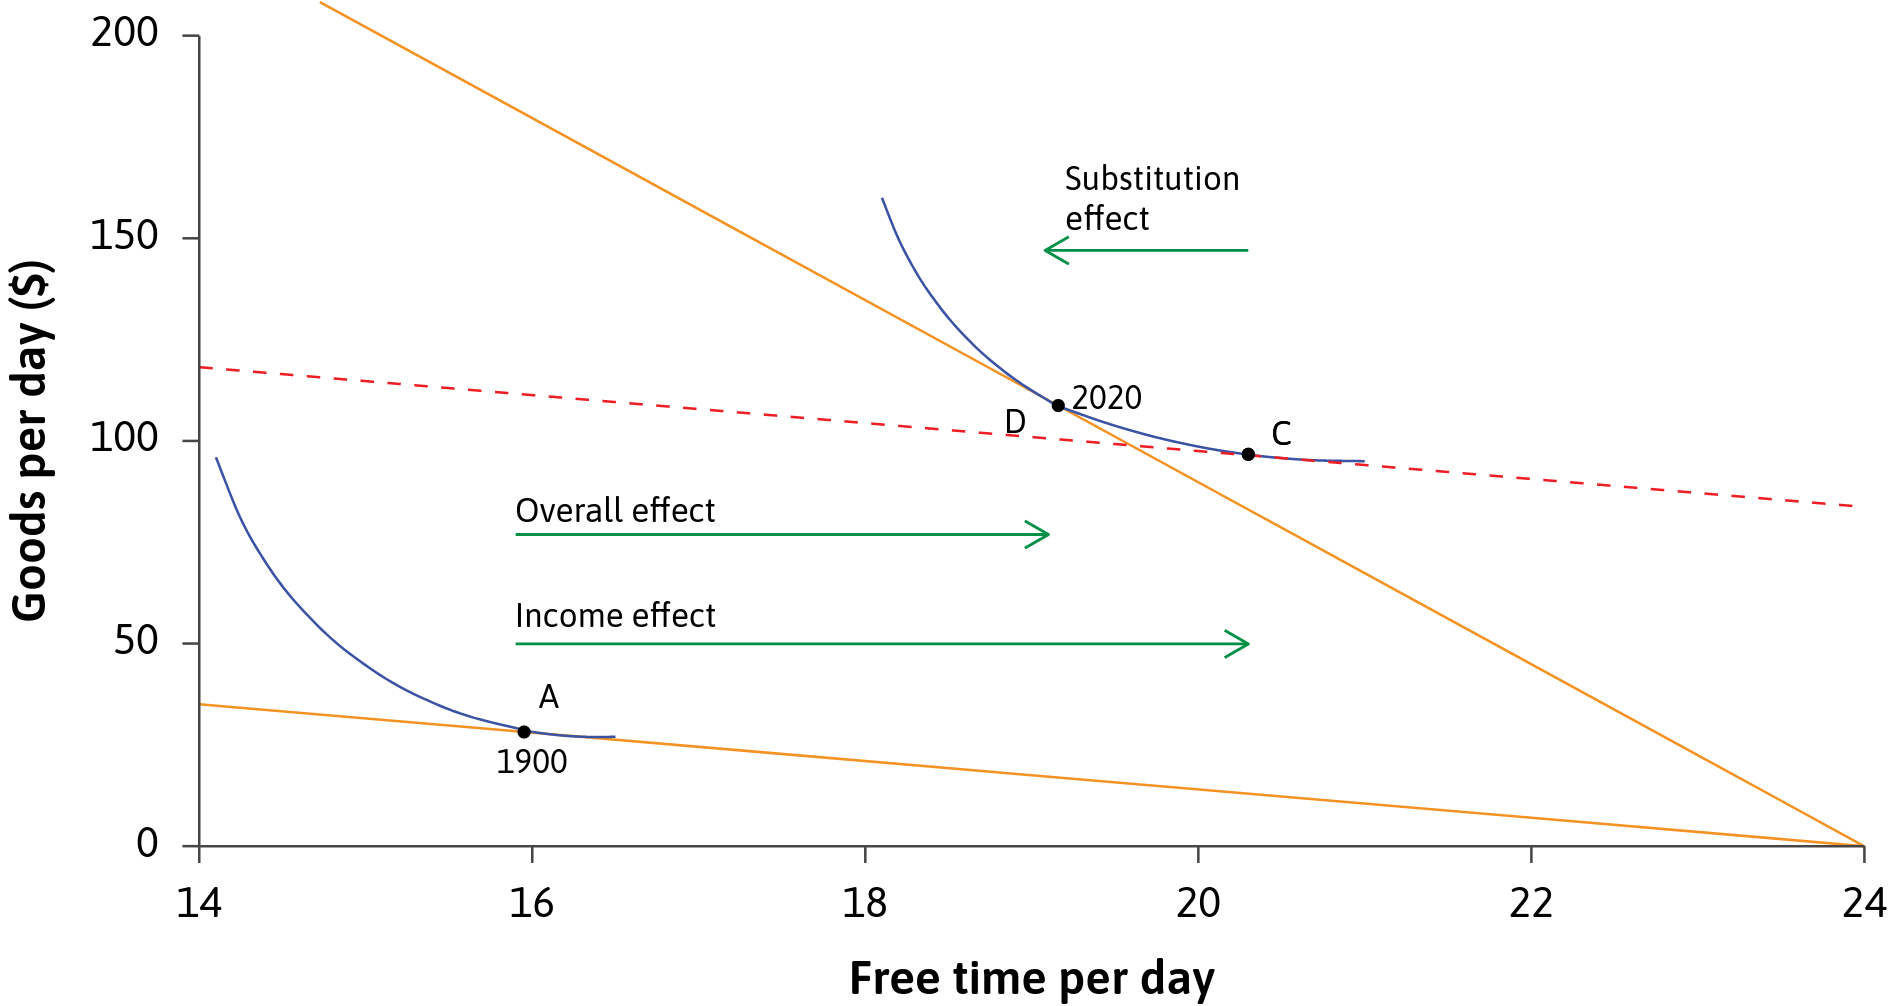
\includegraphics[width=\textwidth]{./figures/WorkdayApplication.png}
    \end{figure}
\end{frame}

\begin{frame}{Difference in Countries}
\label{slide:Difference_in_Countries}
% \url{https://www.core-econ.org/the-economy/book/text/03.html#figure-3-23c}
\begin{figure}
    \centering
    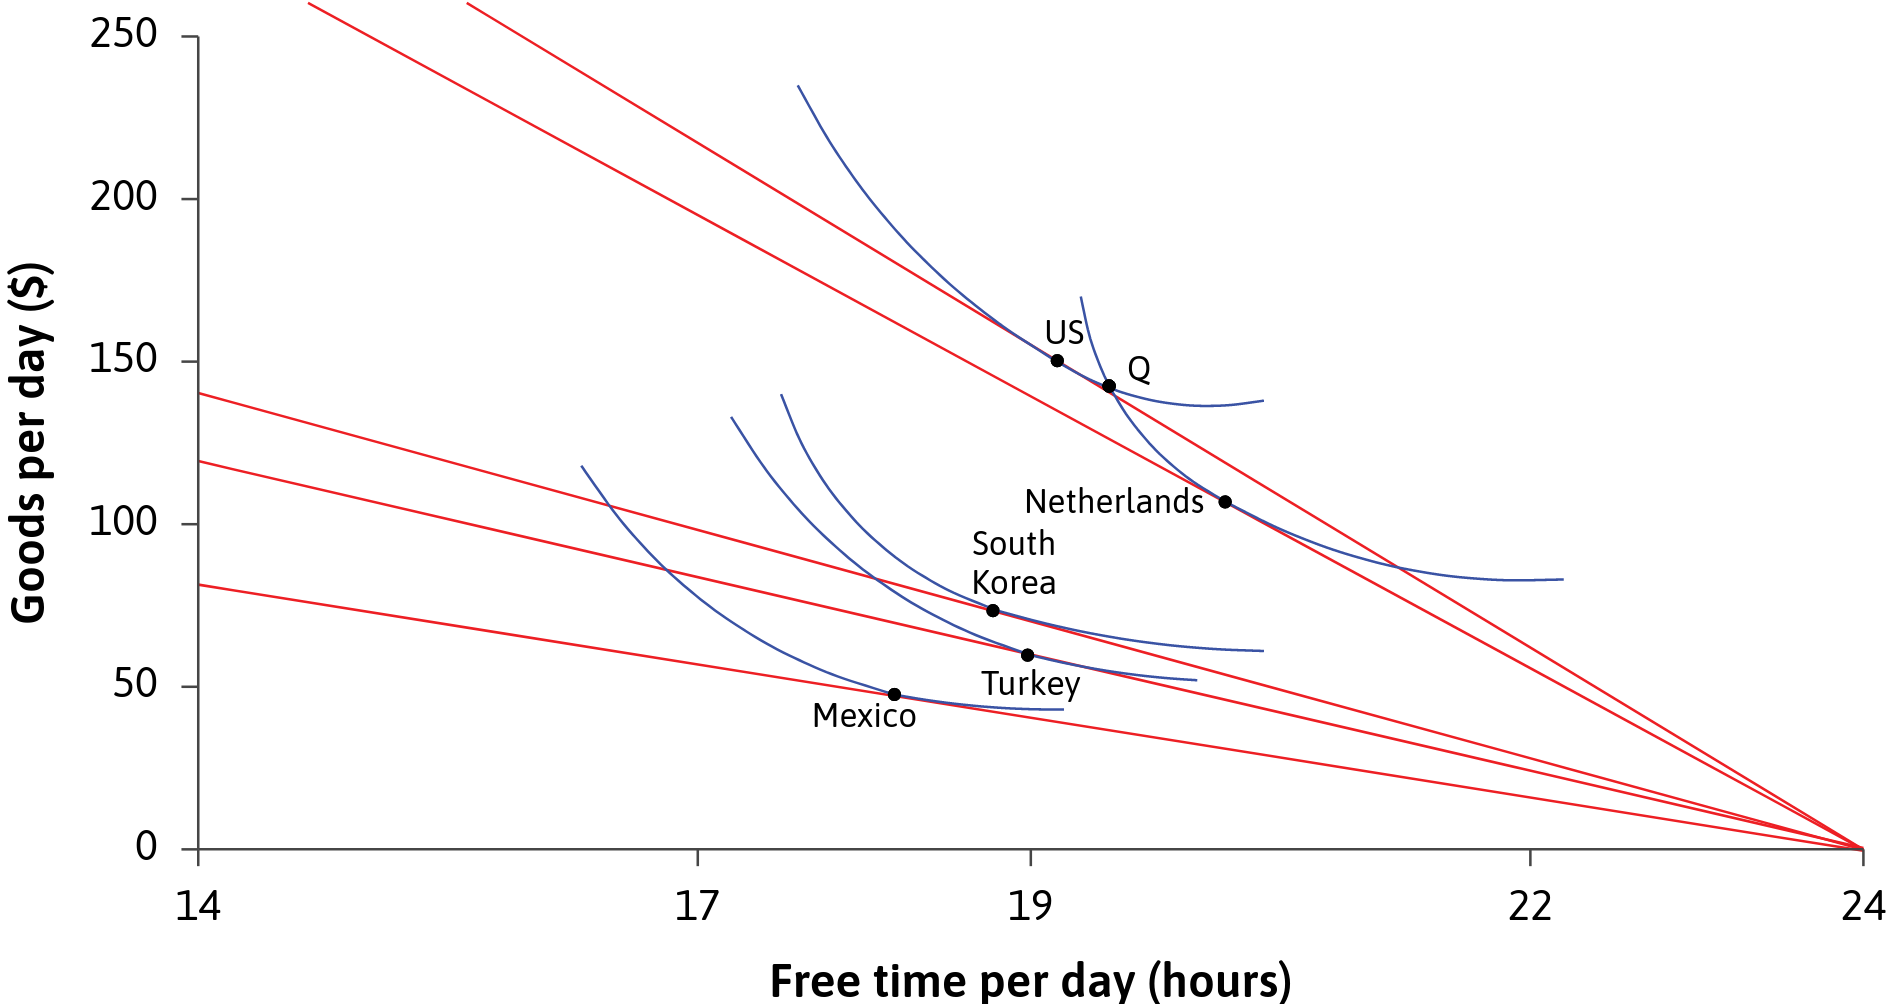
\includegraphics[width=\textwidth]{./figures/WorkCountryDiff.png}
\end{figure}


\end{frame}

\begin{frame}{Good Model?}
\label{slide:Good_Model_}
    Disadvantage:
    \begin{enumerate}
        \item Most people cannot change their working hour in the short term
        \item blame the victim: poor countries are poor because their indifference curve
    \end{enumerate}
    Advantage:
    \begin{enumerate}
        \item Good approximation: Over time, people learn what combination of working hours and free time suits them best.
    \end{enumerate}



\end{frame}


\end{document}
